To attempt at reconstructing the truth from incomplete observations, it is essential to understand the underlying statistics.   Classical and quantum optics provide a comprehensive theoretical foundation to explain photon statistics. For instance, it is well understood that photons from a coherent light source follow a Poisson distribution, often referred to as shot-noise. Whereas, for chaotic (bunched) light, the variance exceeds that compared to their mean, dubbed super-Poissonian. And finally for a squeezed light source, the distribution is sub-Poissonian \cite[Chapter~5]{foxQuantumOpticsIntroduction2006}.

The same principle can be extended to photoelectron emission. For the case of emission events when photons impinge on a material, \citeauthor{mandelFluctuationsPhotonBeams1958} \cite{mandelFluctuationsPhotonBeams1958,mandelFluctuationsPhotonBeams1959} showed that the probability distribution of photoelectron counting follows the photon statistics.

In Section~\ref{sec:poisson-noise-model}, we introduced the assumption that the noise is Poisson distributed. In this chapter, we begin by formally defining the Poisson model for counting photoelectron event data. We examine our data to identify where this model is appropriate and where its limitations become evident. To this end, we introduce some statistical apparatus necessary to estimate parameters and define goodness of model. Further, we explore why the \gls{FEL} light source, as described in Section~\ref{section:light-sources}, exhibits over-dispersed statistics, a characteristic necessitating moving beyond the Poisson model. Accounting for this, we transition to using the Negative Binomial distribution as a more suitable model for the count data.

\section{Theoretical Basis for Poisson Modeling of Photon Detection}\label{section:photon-counting-stats}

Photons are the quantized form of electromagnetic light. They can be thought of as discrete energy packets. The energy of a photon is given by $E = h\nu$, where $h$ is the Planck constant and $\nu$ is the frequency of the light. Due to the discrete nature of photons, it can be shown that the number of photons in a short time interval $\Delta t$ is not constant. These fluctuations are known as photon shot noise.

For a light source with a constant flux\footnote{Flux is the average number of photons passing through the cross-section of a beam per unit time.} $\phi$ such as a single-mode laser, the average number of photons in a beam segment of length is given by $L$, $\lambda = \phi \frac{L}{c}$, where $c$ is the speed of light.

If we subdivide this $L$ into many small intervals  of size $L/N$, where $N$ is large enough so that there is low probability of a photon being in an interval, eventually there will be divisions with no photons, divisions with only single photon, and negligible divisions with multiple photons. For all possible orderings, the probability of finding $n$ subdivisions with a single photon and $(N-n)$ with no photons can be modeled by the Binomial distribution as follows, with $p=\frac{\lambda}{N}$ being the probability of a photon being in a segment:

\begin{equation}
    P(n) = \binom{N}{n} p^n (1 - p)^{N - n}
\end{equation}

Using the Poisson Limit Theorem \cite{fellerIntroductionProbabilityTheory1968}, it can be shown that as $N \to \infty$, and the probability $p \to 0$ such that $Np = \lambda$ remains constant, there is a convergence in distribution to the Poisson distribution.

\begin{note}
    {Poisson distribution}
    The \gls{PMF} for Poisson distribution Poi\((\lambda)\) with \(\lambda > 0\) is defined as
    \begin{equation}
        P(n;\lambda) = \frac{\lambda^n e^{-\lambda}}{n!}, \quad n \in \mathbb{N}_0
    \end{equation}
    \begin{enumerate}
        \item $\lambda = E(X) = Var(X)$ 
        \item Additivity: If $X_1 \sim \text{Poi}(\lambda_1)$ and $X_2 \sim \text{Poi}(\lambda_2)$ are independent Poisson random variables, then the sum $X_1 + X_2$ also follows a Poisson distribution with parameter $\lambda_1 + \lambda_2$
        \begin{equation}
            X_1 + X_2 \sim \text{Poi}(\lambda_1 + \lambda_2).
        \end{equation}
        
        This property is useful when considering counts from multiple independent sources.
    \end{enumerate}
\end{note}

Hence, the Poisson distribution is a suitable model for counting statistics of photons from a coherent light source.

\section{Modelling Photoelectron Statistics}\label{section:photoelectron-counting-stats}
Statistically, a point process is a random collection of points defined on a measure space $(\Omega, \mathcal{A}, \mu)$

\subsection{Doubly stochastic Poisson point process}
Let us define a point process. 

Then poisson point process and inhomogenous poisson point process.

Then cox process or doubly stochastic poisson point process

\begin{figure}
    \centering
    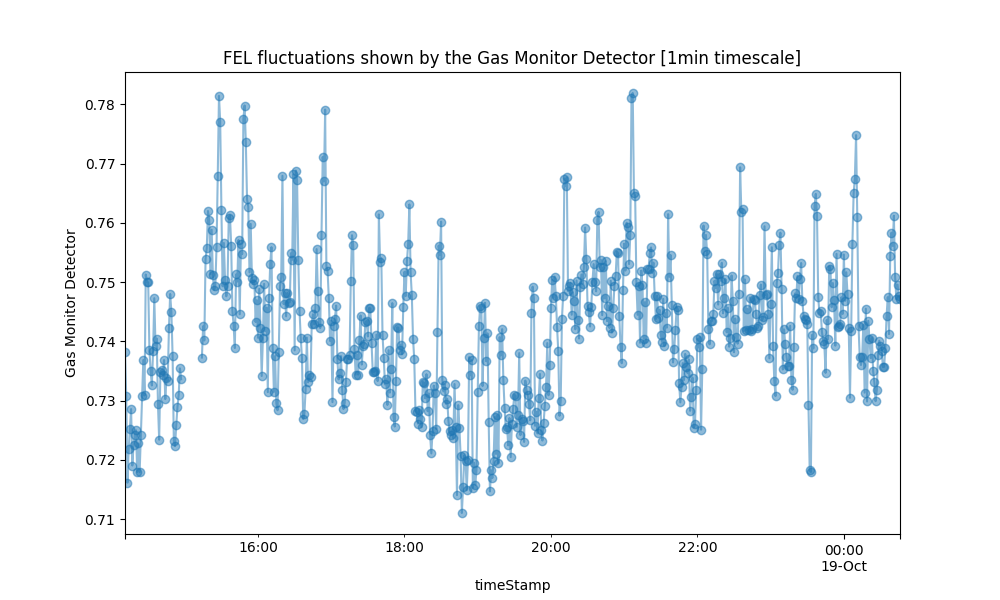
\includegraphics[width=0.7\linewidth]{images/2024-08-16-13-56-32.png}
    \caption{Intensity measurements from the \gls{GMD} over a \qty{30}{hour} time period, window-averaged at \qty{1}{min} intervals. The fluctuations in intensity can be seen, an intrinsic property of the \gls{SASE} process.}
    \label{fig:gmd-intensity}
\end{figure}

\subsection{Photoelectron Counting}
Through usage of only classical arguments, \citeauthor{mandelFluctuationsPhotonBeams1958} \cite{mandelFluctuationsPhotonBeams1958,mandelFluctuationsPhotonBeams1959} derived the probability distribution for photoelectron statistics. We assume that every photoelectron count is a statistically independent event. And for the photoelectron to be ejected in a very short time interval $\Delta t$, the probability should be directly proportional to the intensity of light falling on the detector.

Since the derivation is lengthy, the reader is referred to \cite{mehtaVIIITheoryPhotoelectron1970}, and the results are directly presented.
\begin{note}
    {Probablity distribution of photoelectron counting}
    For a photoelectron detector, the probability of detecting $n$ photoelectrons in a time interval $T$ is given by
    \begin{equation}\label{eq:mandel-photo-electron}
        P(n, t, T) = \int_{0}^{\infty} \frac{\alpha W^n}{n!} e^{-\alpha W} P(W) \, dW
    \end{equation}
    with $\alpha$ being the quantum efficiency, with $W$ being the integrated light intensity ($I$) over the time interval $\Delta t$:
    \begin{equation}
        W = \int_{t}^{t+T} I(t') dt'
    \end{equation}
    and $P(W)$ being the probability density of the random variable $W$.
\end{note}

We can see from \ref{eq:mandel-photo-electron} that even with intensity of light being constant, there are random fluctuations. For a constant intensity light source, the probability distribution simplifies to the Poisson distribution:
\begin{equation}
    P(n, t, T) = \frac{W^n e^{-W}}{n!} 
\end{equation}

This also implies that if there are fluctuations in the intensity of light, the photoelectron counting statistics will deviate from the Poisson distribution. We shall later see that this observation is important to go beyond the Poissonian model in the context of \gls{FEL} light sources.

% Furthermore, in this description, it is assumed a radiation field is on detector system that detects by releases electrons. This is not the case for PES, where the material work function and etc. would make the process dependent on the material.


% The assumption is restrictive because it assumes that the voxels are uncorrelated but in fact thats not the case. this model relies on only counting the electrons but not based on energies and so on.

% There's a lot of parameters that need to be tested to determine what sort of counting statistics the dataset has.

% Controls for the test:
% lets see
% \begin{itemize}
%     \item Total time being looked at (like 1000 s or 20 hours)
%     \begin{itemize}
%         \item distribution might change due to overtime FEL intensity changes
%     \end{itemize}
%     \item Time bins being used (like 2 s vs 20 s and so on).
%     \begin{itemize}
%         \item Seems like distribution changes based on that too
%     \end{itemize}
%     \item Looking at individual pixels on X and Y
%     \item Looking at Energy axis as it behaves weirder
%     \item Looking at a larger region in X and Y 
%     \begin{itemize}
%         \item should follow same statisitics as single pixels
%     \end{itemize}
%     \item Check after removing correlated electrons within each pulse
%     \begin{itemize}
%         \item It is possible that electrons are correlated between different pulses because the time delay is long enough. But seems highly unlikely!
%     \end{itemize}
%     \begin{itemize}
%         \item 
%     \end{itemize}
% \end{itemize}


% \subsection{Before filtering}

% \begin{figure}
%     \centering
%     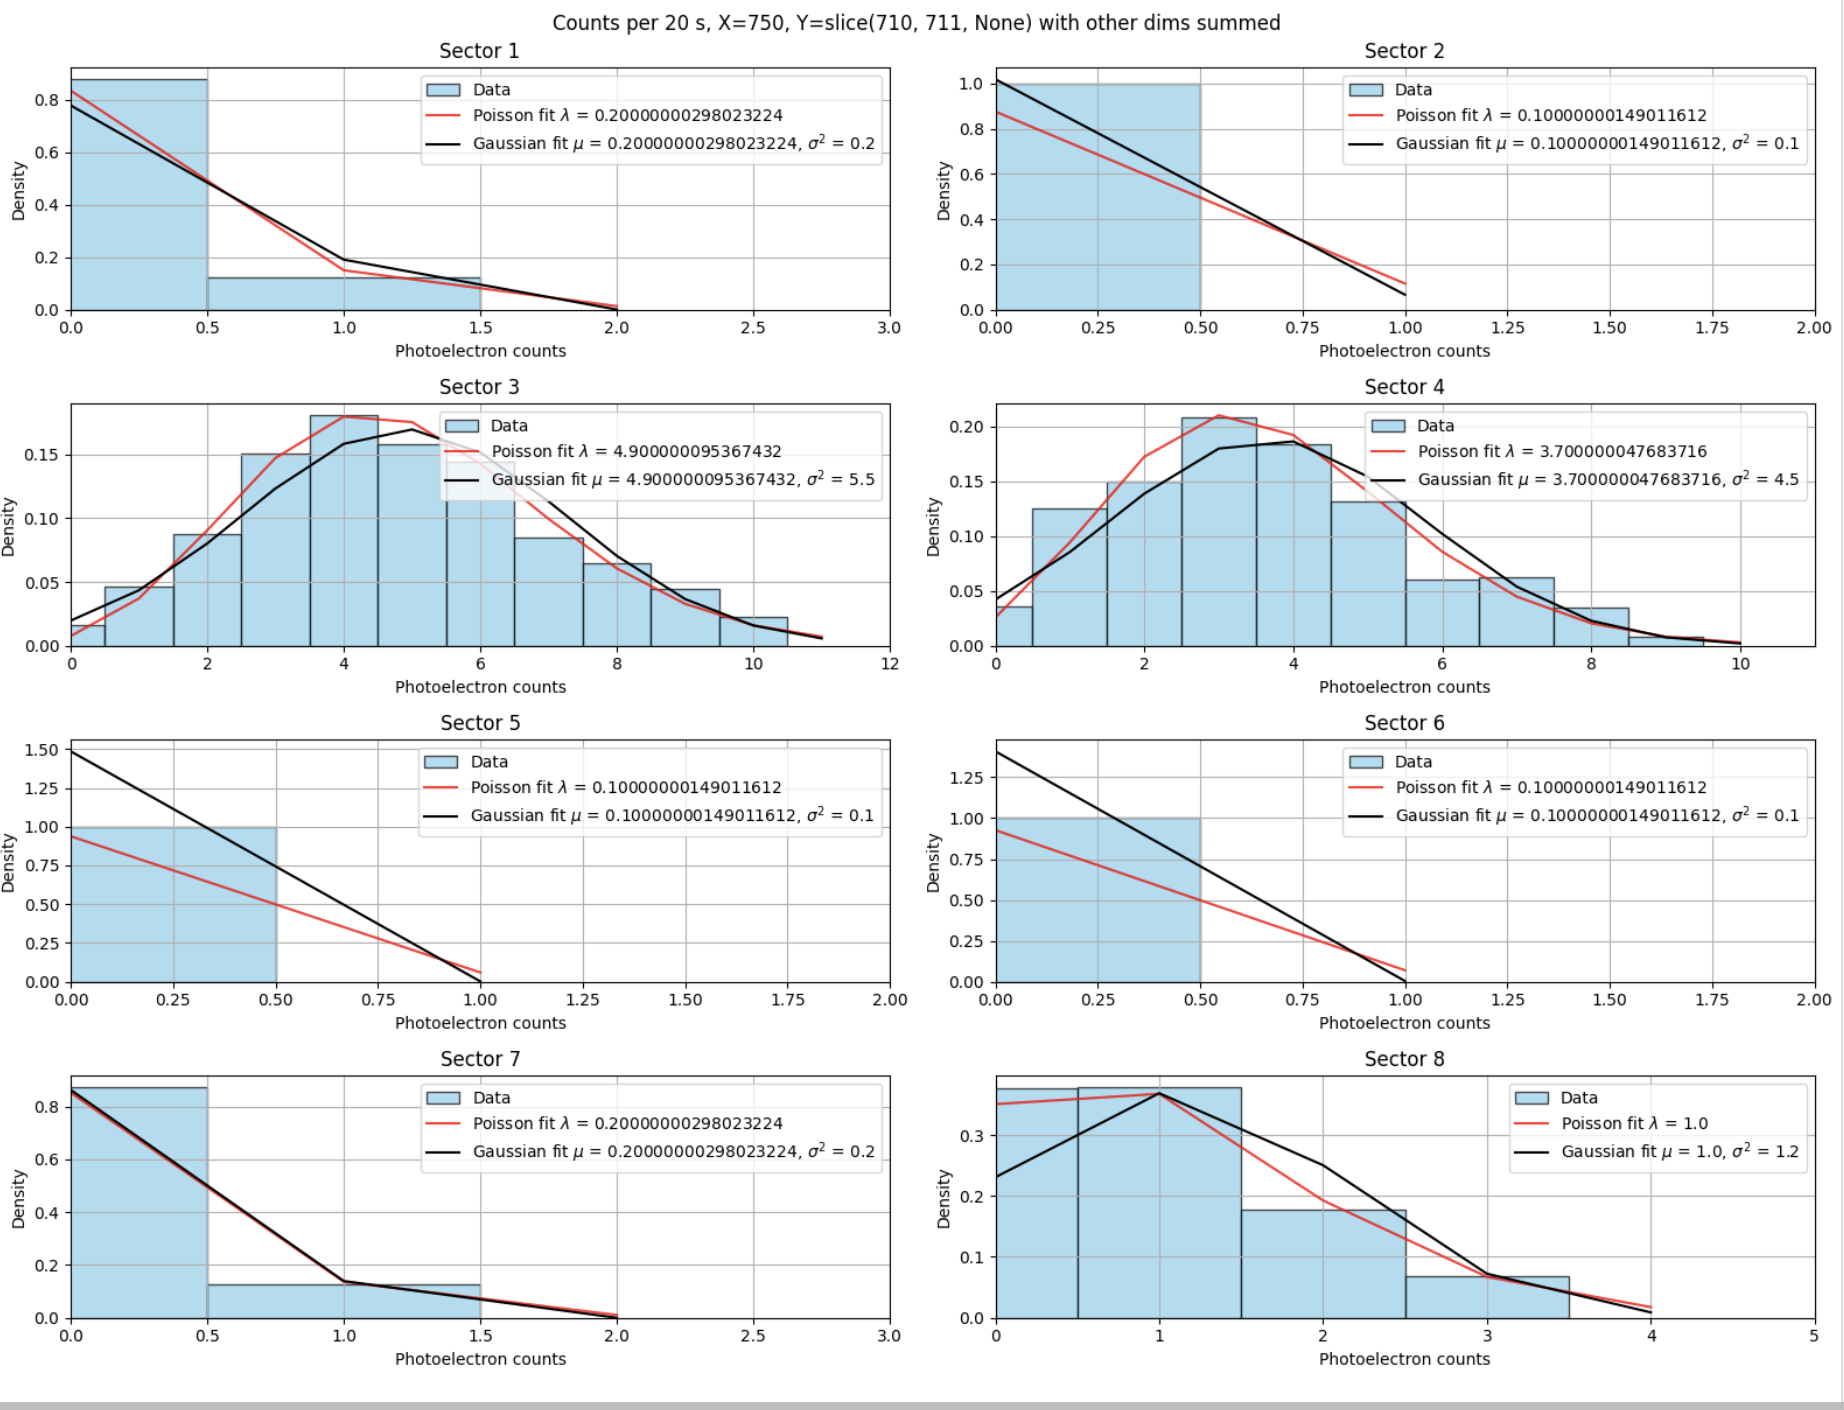
\includegraphics[width=1\linewidth]{images/image.png}
%     \caption{Enter Caption}
%     \label{Image at one 2D pixel but summed over energy}
% \end{figure}

% \begin{figure}
%     \centering
%     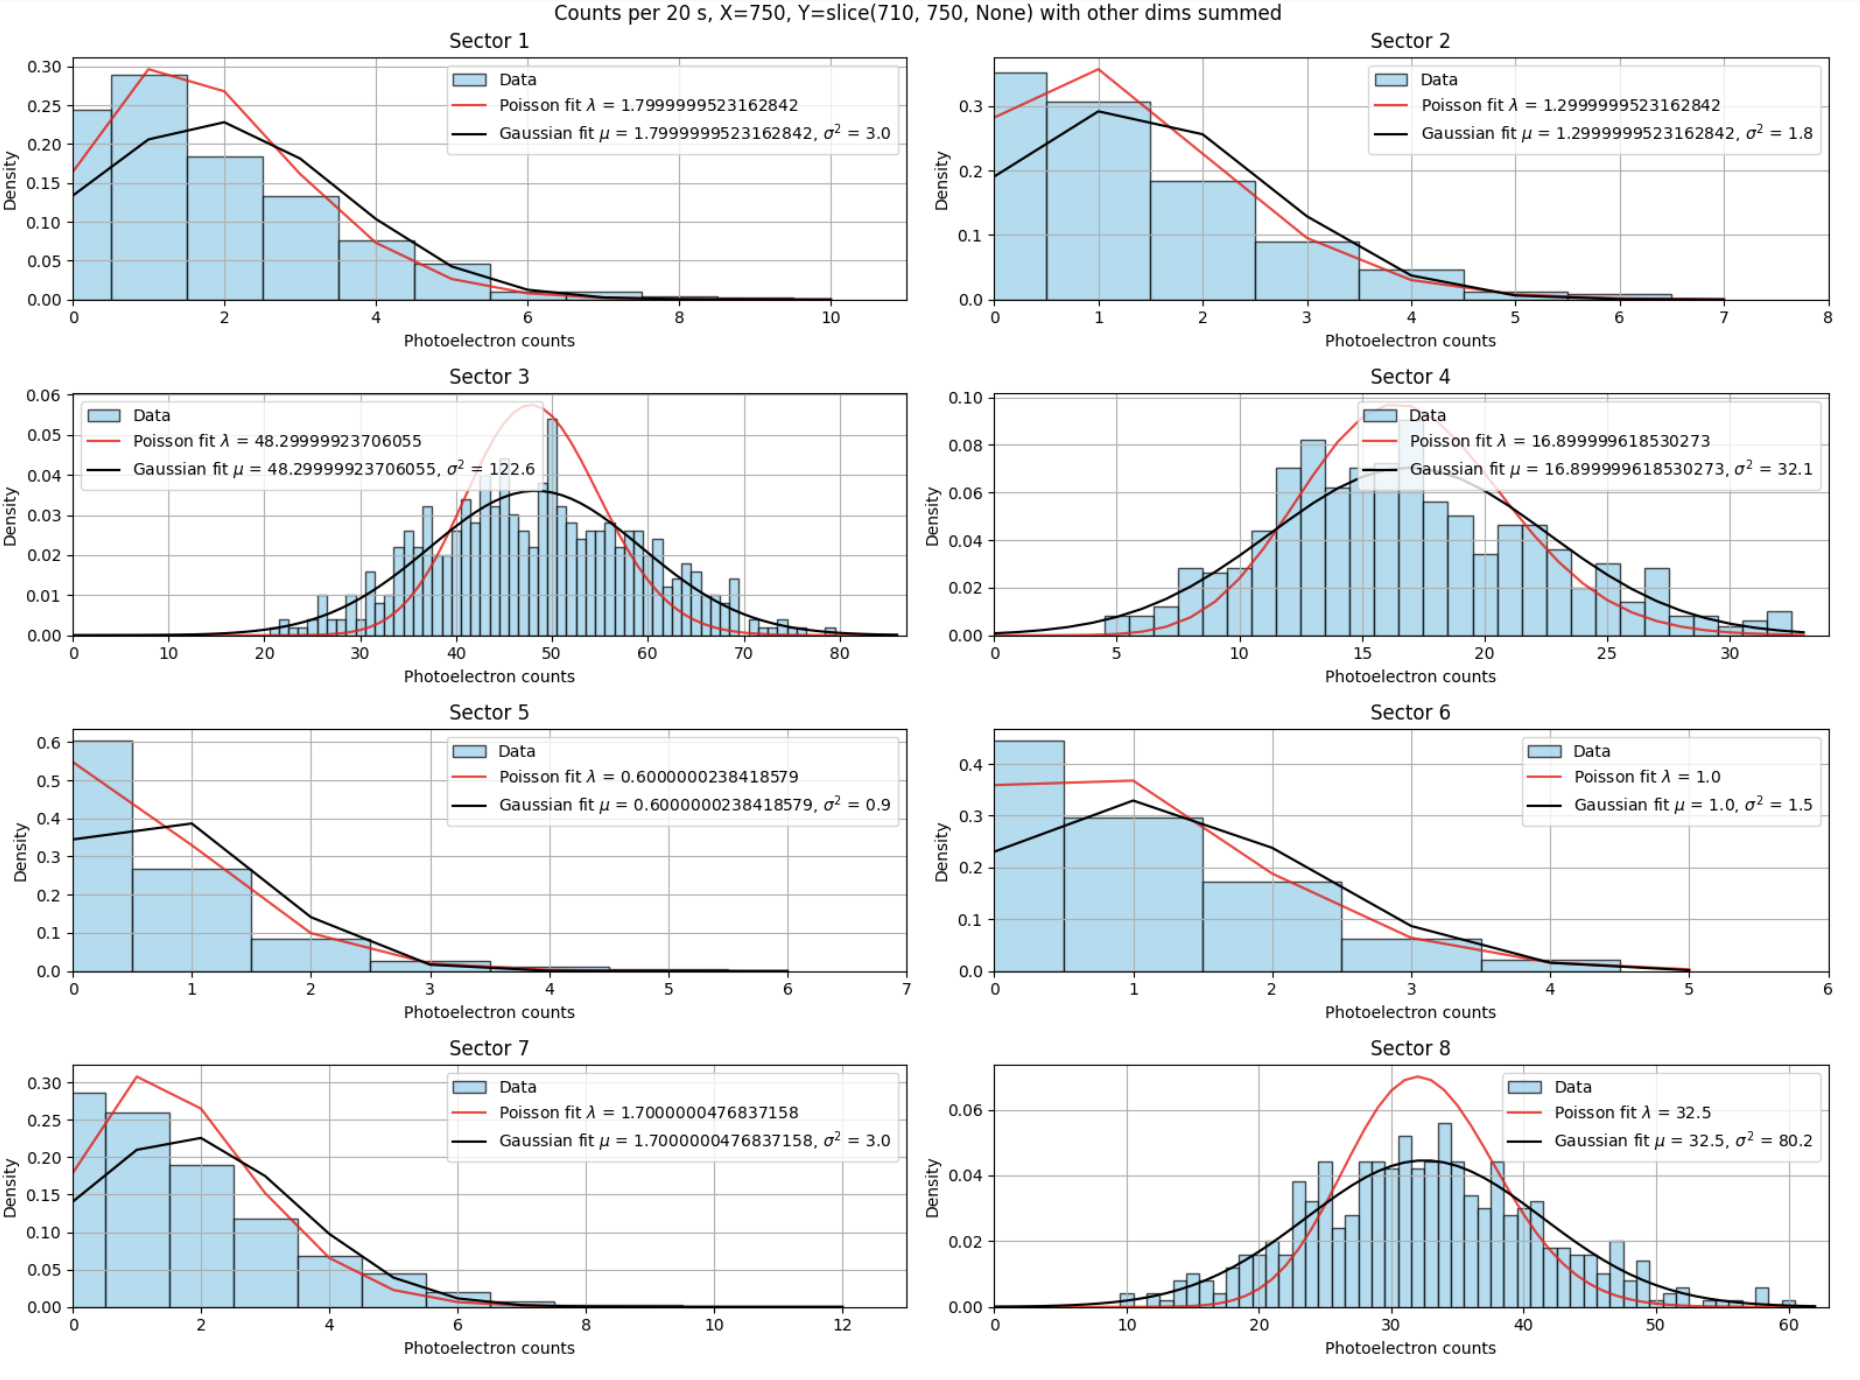
\includegraphics[width=1\linewidth]{images/summed.png}
%     \caption{Image over 40 pixels and summed over energy}
%     % \label{fig:enter-label}
% \end{figure}

% \subsection{After filtering}

% \begin{figure}
%     \centering
%     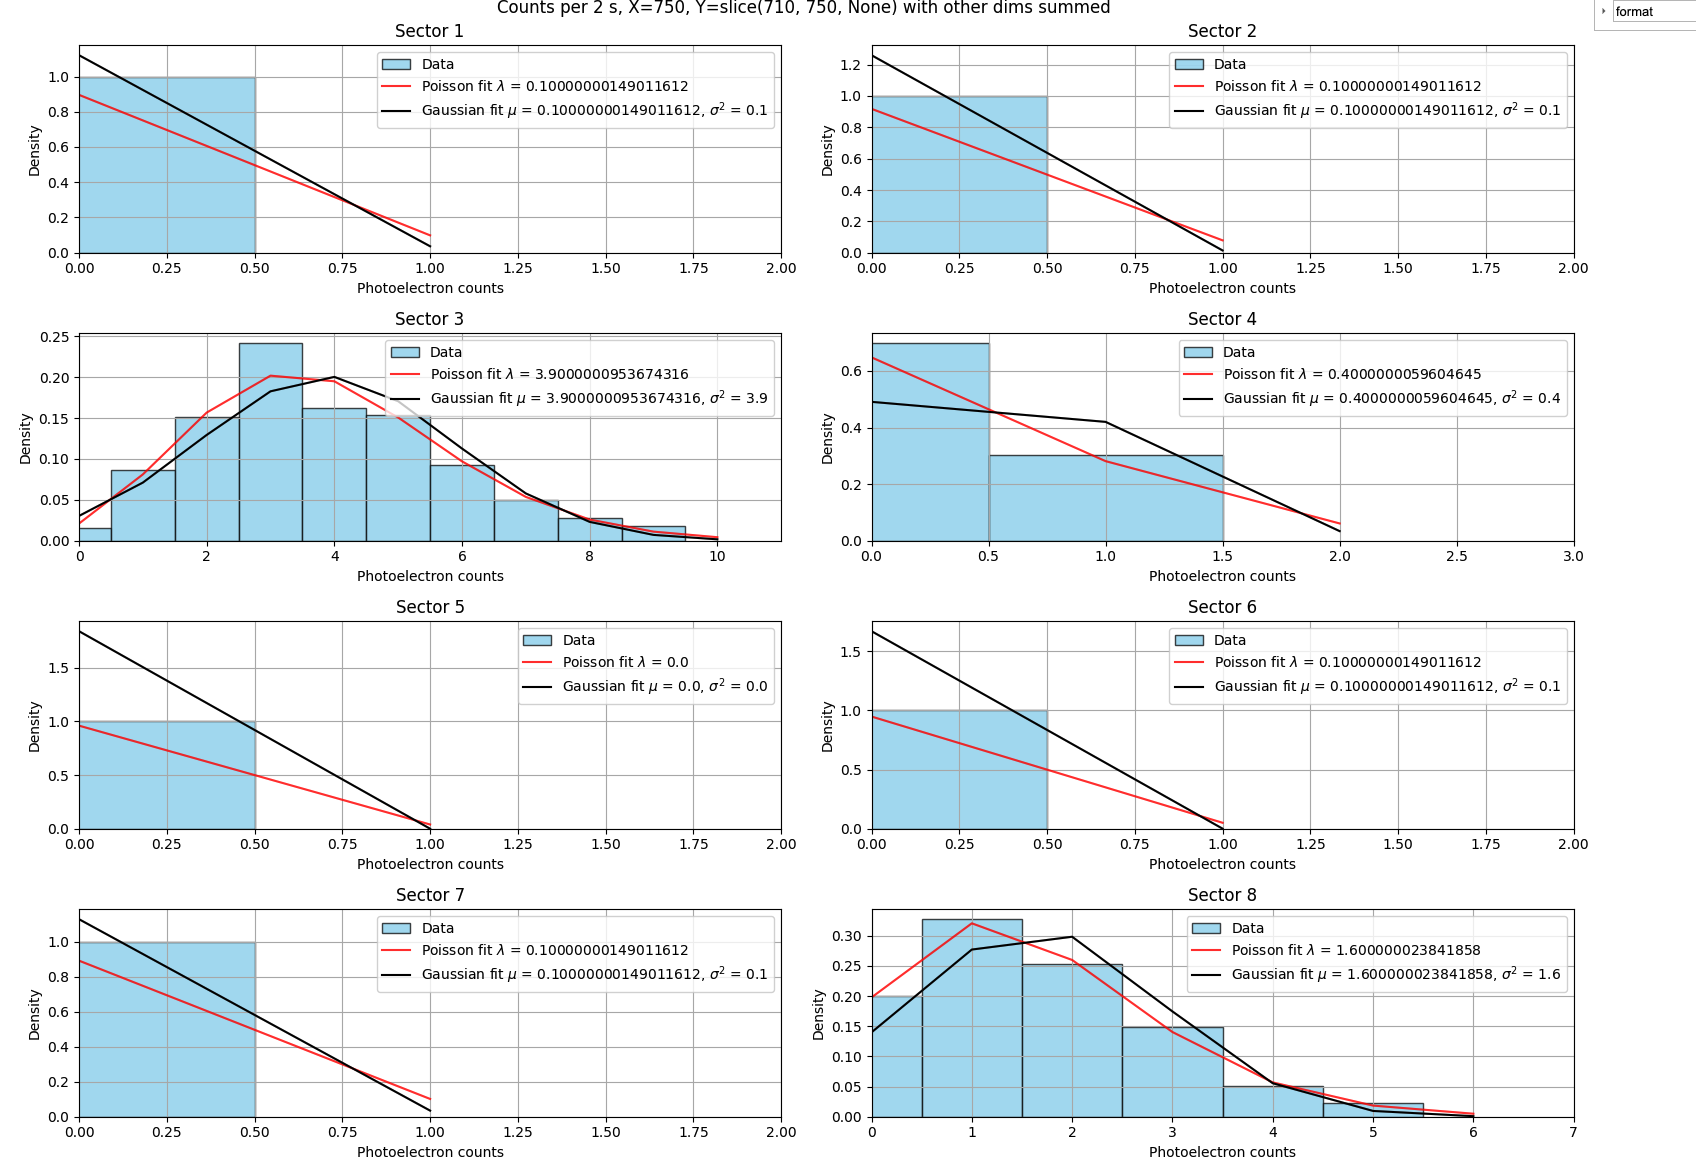
\includegraphics[width=1\linewidth]{images/poisson_stats/after_filtering_region_1000s.png}
%     \caption{Data is filtered here with the KNN and looking at small region}
%     % \label{fig:enter-label}
% \end{figure}

% \begin{figure}
%     \centering
%     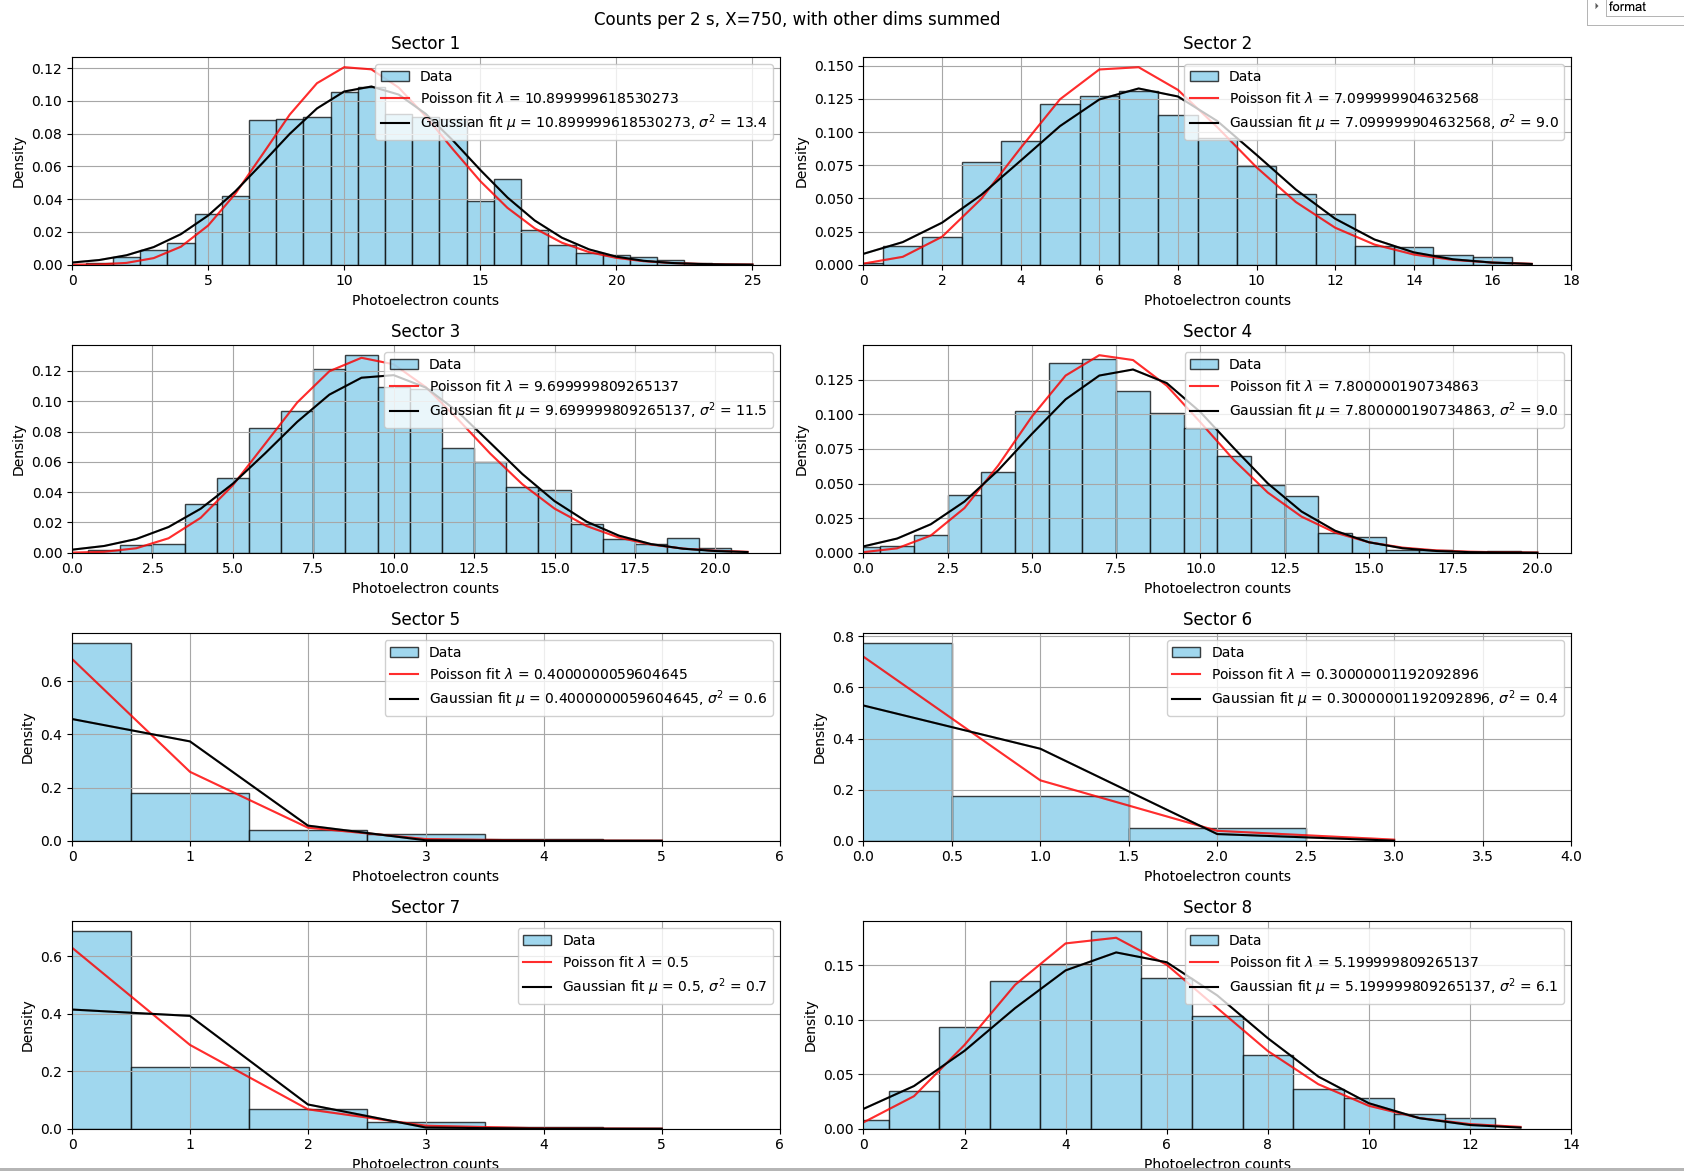
\includegraphics[width=1\linewidth]{images/poisson_stats/filtered_allY_singleX.png}
%     \caption{Enter Caption}
%     % \label{fig:enter-label}
% \end{figure}



% \section{Simulate Noise}
% We simulate the data with Poissonian data.
\section{Statistical testing}

% \begin{figure}
%     \centering
%     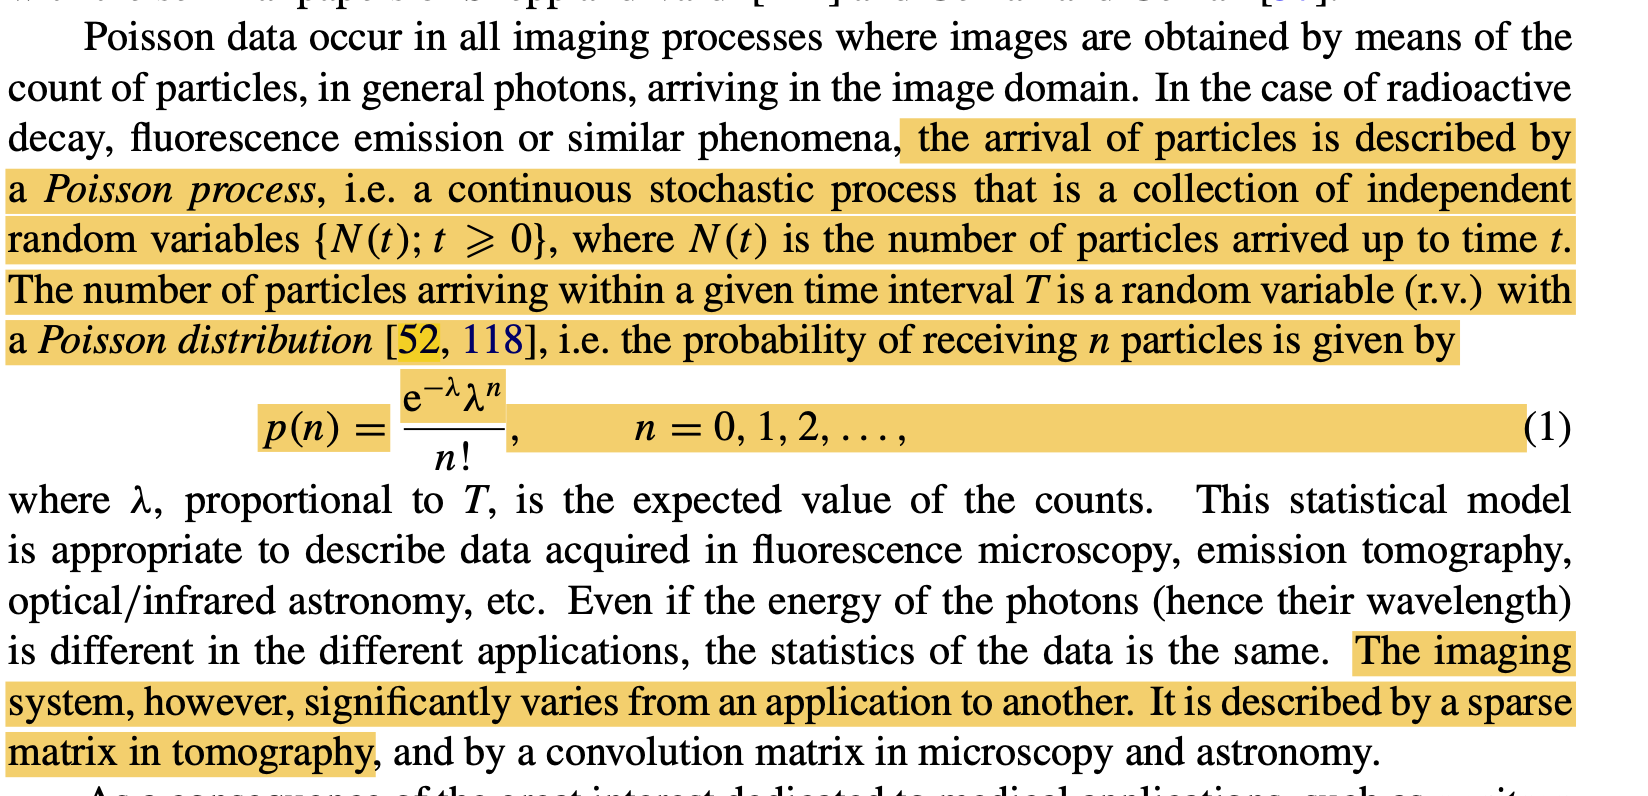
\includegraphics[width=1\linewidth]{images/JD-54-image.png}
%     \caption{Enter Caption}
%     \label{fig:enterl}
% \end{figure}
% Taken from \cite{berteroImageDeblurringPoisson2009} which cites \cite{fellerIntroductionProbabilityTheory1968}


Can't correlate FEL intensity with electron counts per pulse as the GMD is before the monochromator.  \href{https://photon-science.desy.de/facilities/flash/photon_diagnostics/gmd_intensity_and_position/index_eng.html}{description about gmd}

\begin{quotation}
    The physical assumptions which we want to express mathematically are that the \textbf{conditions of the experiment remain constant} in time*, and that non-overlapping time intervals are stochastically independent in the sense that information concerning the number of events in one interval reveals nothing about the other. The theory of probabilities in a continuum makes it possible to express these statements directly, but being restricted to discrete probabilities, we have to use an approximate finite model and pass to the limit.

    Imagine a unit time interval partitioned into n subintervals of length 1/n. A given collection of finitely many points in the interval may be regarded as the result of a chance process such that each subinterval has the same probability $P_{n}$ to contain one or more points of the collection. A subinterval is then either occupied or empty, and the assumed independence of non-overlapping time intervals implies that we are dealing with Bernoulli trials: We assume that the probability for exactly k occupied subintervals is given by $b(k;n,P_{n})$. We now refine this discrete model indefinitely by letting n→inf. The probability that the whole interval contains no point of the collection must tend to a finite limit. But this is the event that no cell is occupied, and its probability is $(1-p_{n})^{n}$. Passing to logarithms it is seen that this quantity approaches a limit only if $np_{n}$
    from book \cite{fellerIntroductionProbabilityTheory1968}
\end{quotation}



\section{Poisson Process testing}

\begin{figure}[h]
    \centering
    % First subfigure (Hyperparameter Search with Averaged 10 Images using MS-SSIM)
    \begin{subfigure}[t]{0.49\linewidth}
        \centering
        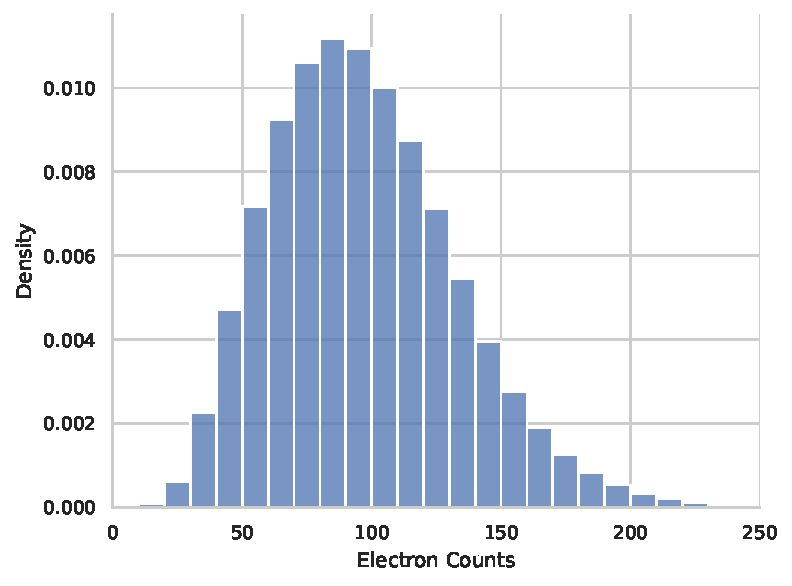
\includegraphics[width=\linewidth]{images/hist_counts_per_train.pdf}
        \caption{}
        \label{fig:hist-grir-flash}
    \end{subfigure}
    \hfill
    % Second subfigure (Hyperparameter Search with Averaged 10 Images using Sigma)
    \begin{subfigure}[t]{0.49\linewidth}
        \centering
        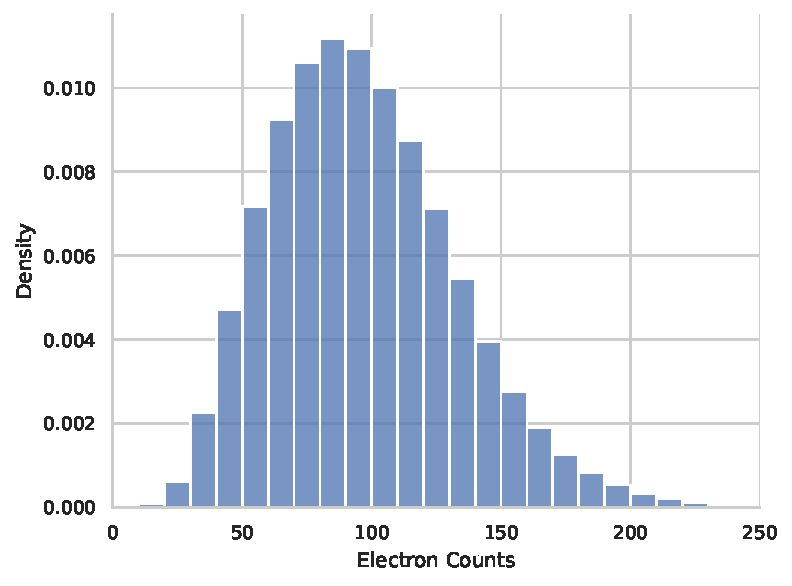
\includegraphics[width=\linewidth]{images/hist_counts_per_train.pdf}
        \caption{}
        \label{fig:hist-wse2-laser}
    \end{subfigure}
    \caption{}
    \label{fig:}
\end{figure}


We test with two datasets, measured with different light sources: \gls{WSe2} measured with a pulsed laser, and \gls{GrIr} measured with an \gls{FEL}. As seen from the theoretical standing, the statistics from a laser source should be explainable using a homogenous poisson point process, and temporally they should follow a Poisson distribution.
Whereas, the \gls{FEL} source has intensity fluctuations and the expectation is that the statistics should be over-dispersed. Since the intensity variations are themselves random, the cox process is an appropriate model.

Important to note is that the point process is temporally defined and not spatially, meaning that the data points should not be distributed with poisson statistics in space. The data points are not independent in space, as the photoelectrons are ejected from the same material and are correlated. Otherwise, there would be little point to do \gls{PES}.
However, due to sparse data, it becomes necessary to look at small regions, hoping the nearby points are similar enough to not affect the statistics.

The ideal situation would be specially designed experiment that exhibits no spatial correlations and with long enough acquisition time to get a good estimate of the statistics at different time windows.

There are two ways to test the point process. One is to look at the time intervals between events, and the other is to look at the number of events in a fixed time interval. While the light sources give timing information coarser than the electron detection time, the \gls{DLD} detector provides the exact time of arrival of each electron. Hence, the independence of the events can be tested by looking at the time intervals between events.

\subsection{Time intervals between events}


\subsection{Number of events in a fixed time interval}
Testing with small time intervals, we can see that the data follows a Poisson distribution.

However, as we increase the time window, the data starts to deviate from the Poisson distribution. As more events accumulate in the region, the underlying spatial correlations become apparent and start to affect the statistics. The spatial intensity variantions. Then we could describe the process as an inhomogenous poisson process with the spatial intensity determined by the material properties

In practice, it is difficult to test the point process directly. 

As seen in \cref{sec:dld}, special care needs to be taken to draw conclusions using single event data from detector.
We only look at a single sector as we know the two sectors have repeated counts.
Considering the data acquisition scheme of having a pulse and then not, if we try to access the process by taking time intervals, it wouldnt make sense. better would be to look at the data in terms of pulses.
Or we can avoid this issue by looking at time scales above the trainId time scale, where each train comes every 100 ms.
Let us start by looking at the \gls{GrIr} single event data. Ideal would be to look at individual voxels but the counts are way too low so We start by looking at a single dimension, the  axis

To make sure spatial correlations don't impact the statistics, we can look at a 3D patch that is small.

Also interesting to see two pixels at different locations

\section{Chi-squared Goodness of Fit Test}
We hypothesize that the data follows a certain distribution e.g. Poisson, Normal, Negative Binomial The Chi-squared Goodness of Fit Test is used to determine if the observed data is consistent with the expected distribution.

Let \( X_1, X_2, \ldots, X_n \sim \text{i.i.d. } F \) and \( Y_1, Y_2, \ldots, Y_m \sim \text{i.i.d. } G \), where \( F \) and \( G \) are strictly increasing continuous \glsplural{CDF}.

The hypotheses for the chi-square test are:

\begin{equation}
    H_0: F = G \leftrightarrow   H_1: F \neq G
\end{equation}
The hypothesis test for the Poisson distribution is the Chi-squared Goodness of Fit Test. The test statistic is given by:

\begin{equation}
    \chi^2 = \sum_{i=1}^{k} \frac{(O_i - E_i)^2}{E_i}
\end{equation}
where \(O_i\) is the observed frequency and \(E_i\) is the expected frequency. The degrees of freedom are given by \(k-1\), where \(k\) is the number of bins.

For goodness-of-fit tests, small p-values indicate that you can reject the null hypothesis and conclude that your data were not drawn from a population with the specified distribution. Consequently, goodness-of-fit tests are a rare case where you look for high p-values to identify candidate distributions. 
(From \href{https://statisticsbyjim.com/hypothesis-testing/goodness-fit-tests-discrete-distributions/}{This website})


\begin{figure}[t]
    \centering
    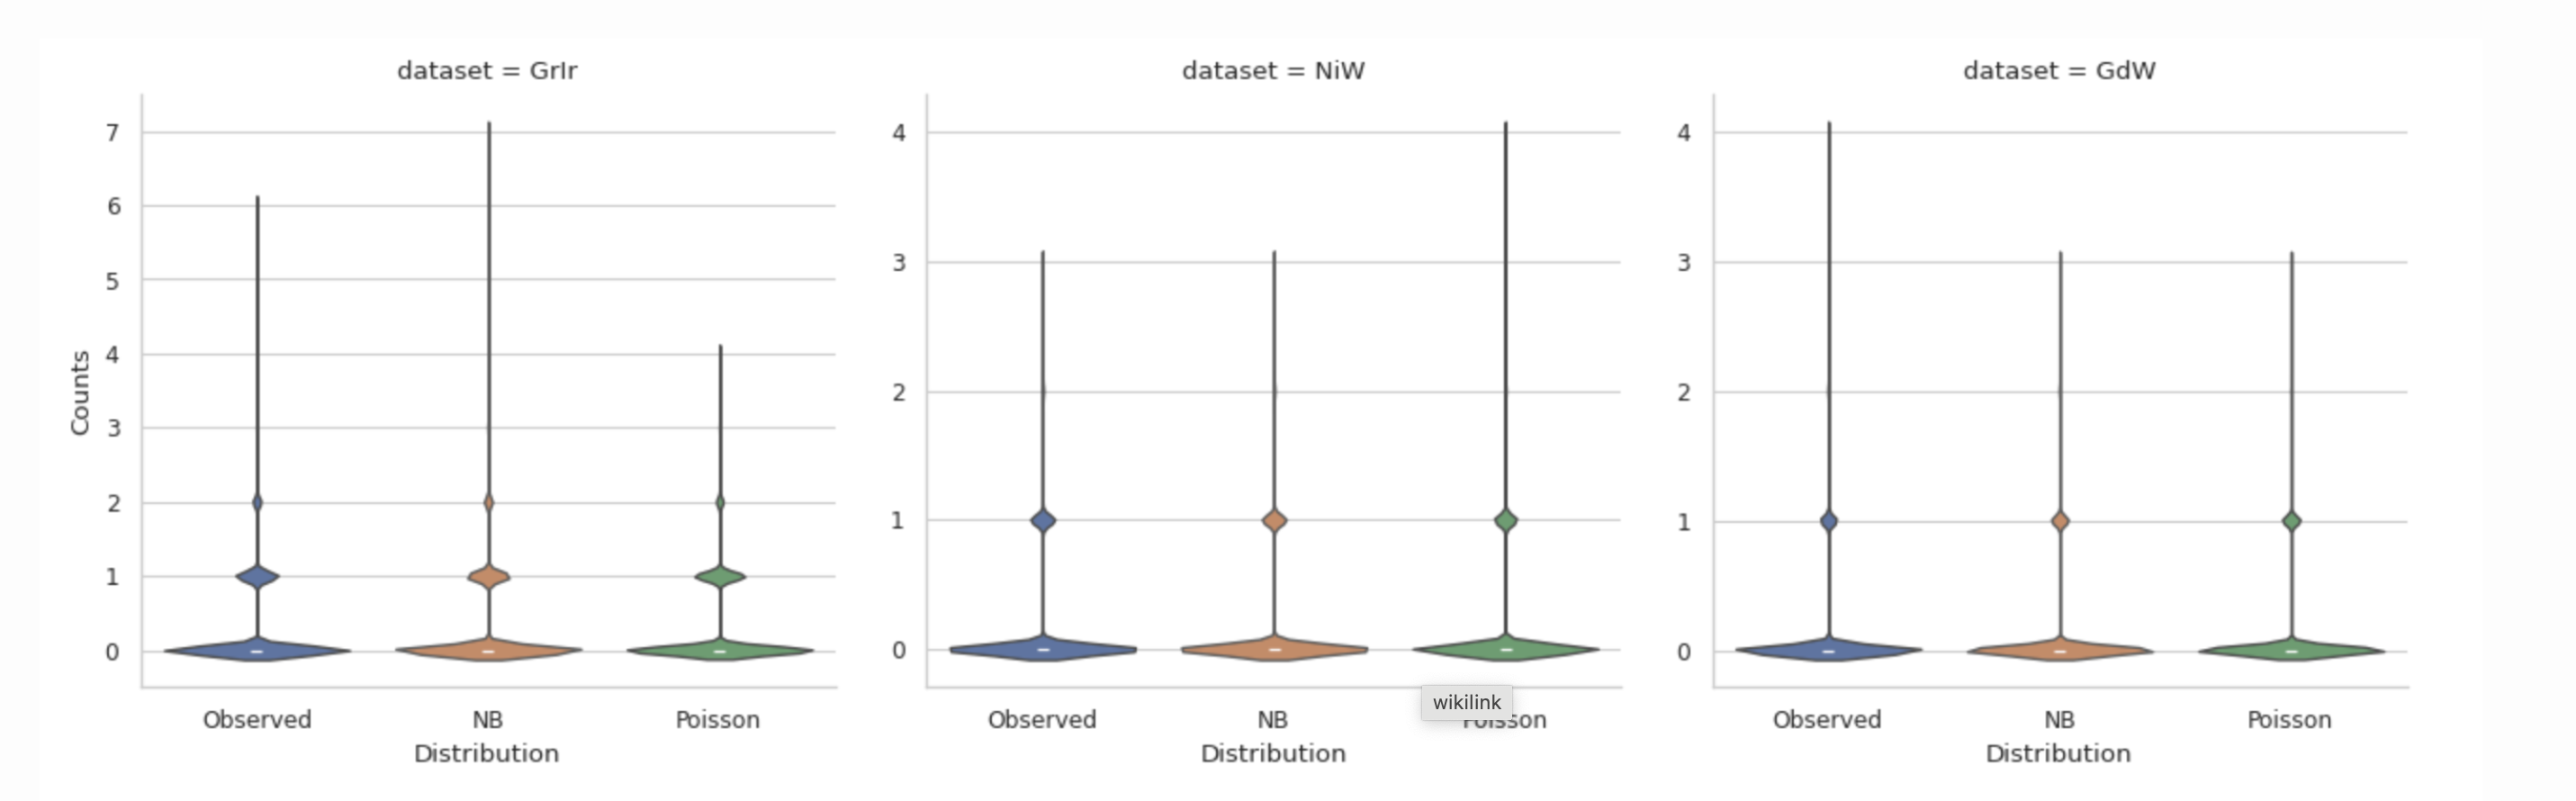
\includegraphics[width=1\linewidth]{images/violin_plots_per_pulse.png}
    \caption{Enter Caption}
\end{figure}

\begin{figure}[htbp]
    \centering
    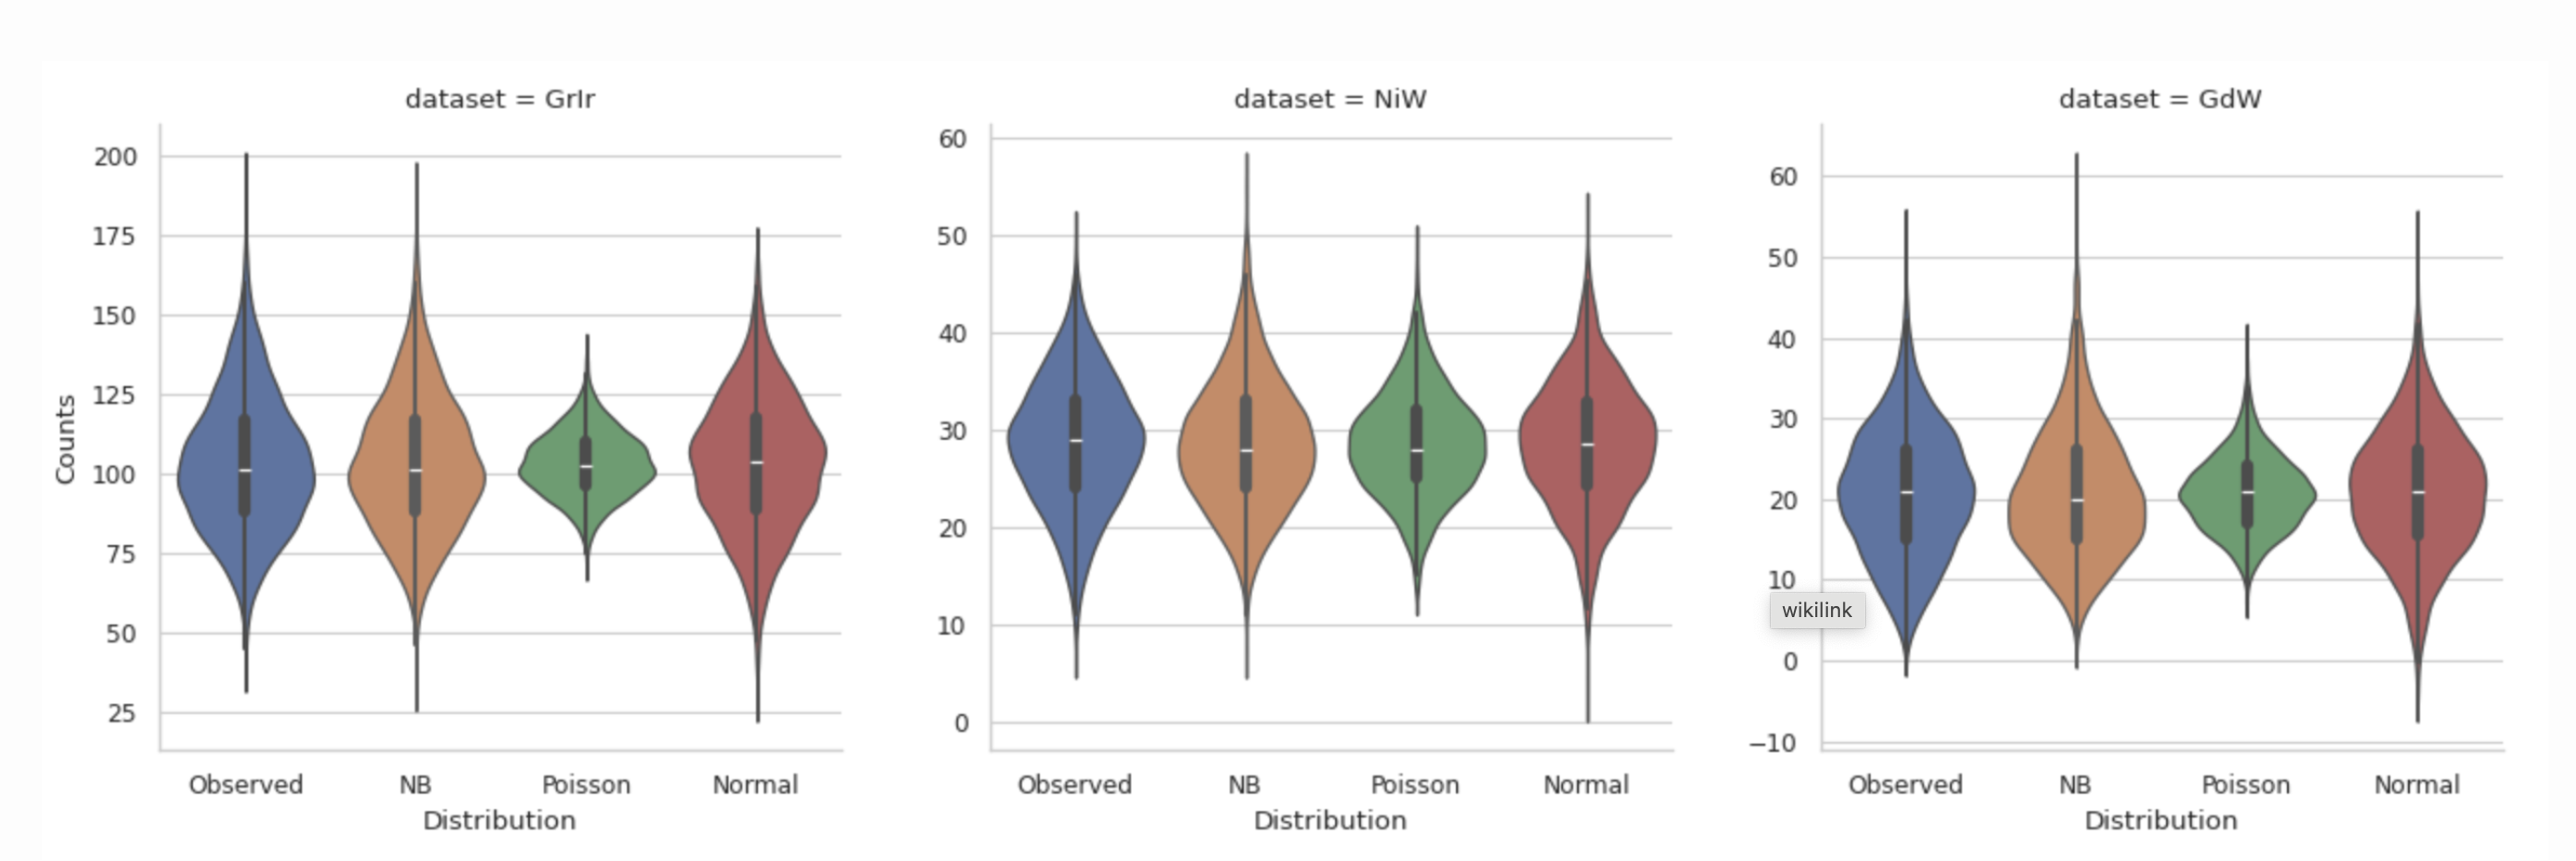
\includegraphics[width=1\linewidth]{images/violinplots_per_train.png}
    \caption{ss}
    \label{s}   
\end{figure}
\section{Modeling over-dispersed count data}

\section{The SASE process as an explanation of over-dispersed statistics}
